%%% Sample LaTeX file for Physics 107
%%% I (M.S.-S.) typically edit in TeXworks and use pdfLaTeX as the typesetting engine

\documentclass[twocolumn,aps,prl]{revtex4-1} % For final two-column format
%\documentclass[twocolumn,aps,prl]{revtex4-1} % For double-spaced, single-column draft

\usepackage{graphicx}% Include figure files
\usepackage{amsmath,amssymb,comment,float, subfig, adjustbox, mathtools}
\usepackage{courier}
\usepackage{hyperref}

% It may be convenient to define shortcut commands such as these:

\newcommand{\ket}[1]{\ensuremath{\vert #1 \rangle}}
\newcommand{\abs}[1]{\ensuremath{\vert #1 \vert}}
\renewcommand{\vec}[1]{\ensuremath{\mathbf{#1}}}
\newcommand{\uvec}[1]{\ensuremath{\hat{\vec{#1}}}}
\newcommand{\squeezeup}{\vspace{-2.5mm}}
\newcommand{\pdd}[2]{\frac{\partial #1}{\partial #2}}
\newcommand{\pd}[1]{\frac{\partial}{\partial #1}}
\newcommand{\psdd}[2]{\frac{{\partial}^2 #1}{\partial {#2}^2}}
\setlength{\parskip}{0pt}

\usepackage[margin=10pt,font=small,labelfont=bf, justification=raggedright]{caption}

\begin{document}
\raggedbottom

\title{Simulating Liquid Crystals}

\author{Aaron Reed}
\affiliation{Department of Physics, Stanford University, Stanford, California 94305, USA}
\date{\today}

\begin{abstract}
I simulate the response of liquid crystal molecules to the electric field of an azimuthally symmetric capacitor.
\end{abstract}

\maketitle

\section{Introduction -- Liquid Crystals}

\subsection{History}
The first liquid crystal, cholesteryl benzoate, was identified by Austrian botanical physiologist Friedrich Reinitzer and further characterized by German physicist Otto Lehmann. \cite{dunmur_soap_2011} Reitnizer observed that the substance had two melting points: it melted from a solid into a cloudy liquid at 418.7 K, and melted again into a clear liquid at 451.7 K (Fig. \ref{fig:LC_tube}).  He also found that the cloudy phase reflected circularly polarized light and could change the polarization of light, while the clear phase had the properties of an isotropic liquid.  Lehmann observed that the cloudy phase contained crystallites and exhibited birefringence like a crystalline solid, so he dubbed the material a \textit{liquid crystal}.

Later, French physicist Georges Friedel proposed the categorization of liquid crystal phases into nematic, smectic, and columnar phases that is still in use today.  Charles Maugin, also French, discovered that liquid crystals change their alignment in response to applied electric or magnetic fields.  Between the 1960s and 1990s, Pierre-Gilles de Gennes of France and Frank M. Leslie of Scotland further developed the theory of liquid crystals, and RCA Laboratories developed liquid crystal displays.

\begin{figure}
    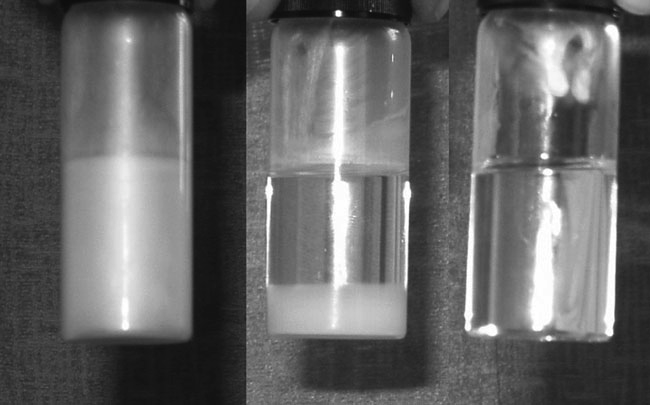
\includegraphics[width=\columnwidth]{LC_tube.png}
    \caption{\textbf{Double melting:} \cite{dunmur_soap_2011} A vial of liquid crystal being warmed from room temperature.  A phase transition from liquid crystal (opaque) to isotropic liquid (clear) appears at the upper surface of the liquid and moves downward.}
    \label{fig:LC_tube}
\end{figure}


\subsection{Formal Definition}

A liquid crystal can be formally defined using the density-density correlation function $\langle\rho(\mathbf{x})\rho(\mathbf{x}_0)\rangle$ of statistical mechanics. \cite{gennes_physics_1974}  Let $\mathbf{x}_0$ be the position of a molecule or some other feature; roughly speaking, the correlation function gives the probability of finding an equivalent molecule or feature at position $\mathbf{x}$.

\begin{figure}
    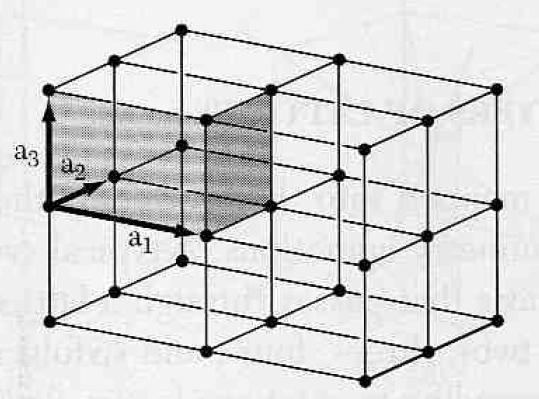
\includegraphics[width=\columnwidth]{unit_cell.png}
    \caption{\textbf{Unit cell:} \cite{kittel_introduction_2005} In a crystal, the smallest repeating unit that has the full symmetry of the crystal is called the unit cell.  In this cubic lattice, it is the parallelepiped formed by basis vectors $\mathbf{a}_1$, $\mathbf{a}_2$, and $\mathbf{a}_3$. }
    \label{fig:unit_cell}
\end{figure}

A crystal is defined by the fact that it is periodic in space, that is, a feature found at $\mathbf{x}_0$ is also found at all positions $\mathbf{x} = \mathbf{x}_0 + n_1 \mathbf{a}_1 + n_2 \mathbf{a}_2 + n_3 \mathbf{a}_3$ for $n_i$ integers and $\mathbf{a}_i$ basis vectors  (Fig. \ref{fig:unit_cell}).  Thus, in a crystalline solid, the correlation function retains space periodicity at arbitrary distance from $\mathbf{x}_0$:

\begin{equation*}
\begin{split}
    \lim_{|\mathbf{x}-\mathbf{x}_0|\to \infty} \langle\rho(\mathbf{x})\rho(\mathbf{x}_0)\rangle = F(\mathbf{x} - \mathbf{x}_0)
\end{split}
\end{equation*}

\noindent where $F$ is periodic in the basis vectors $\mathbf{a}_i$.

On the other hand, in an isotropic liquid the correlation function tends toward a constant, the square of the average density $\bar{\rho}$:

\begin{equation*}
\begin{split}
    \lim_{|\mathbf{x}-\mathbf{x}_0|\to \infty} \langle\rho(\mathbf{x})\rho(\mathbf{x}_0)\rangle \simeq \bar{\rho}^2
\end{split}
\end{equation*}

\noindent Note that in an isotropic liquid, there is a length scale $\xi$ over which correlations decay.  (X-ray diffraction of isotropic liquid results in diffuse peaks of typical width $\xi^{-1}$.)

A liquid crystal (LC) is \textit{a system in which a liquid-like order exists in at least one direction of space and in which some degree of anisotropy is present.}\citep{gennes_physics_1974}  By `some degree of anisotropy,' we mean that the LC has a correlation function that depends not solely on the magnitude of $(\mathbf{x} - \mathbf{x}_0)$, but also on its direction.



\subsection{Types of Liquid Crystals}

The nature of the anisotropy in an LC determines its classification into one of several \textit{mesophases} between crystalline solid and isotropic liquid; several distinct mesophases can exist between the two extremes. (Fig. \ref{fig:phases}) Phase transitions are called \textit{thermotropic} if they occur with changing temperature and \textit{lyotropic} if they occur with changing LC molecule concentration in the solvent.  The three known types of LC mesophases are \textit{nematic}, \textit{smectic}, and \textit{columnar}.

\subsubsection{Nematics}

In \textit{nematic} phases, the only difference from the isotropic liquid is that there are two distinct length scales, $\xi_\parallel$ and $\xi_\perp$, over which the correlation function decays at different rates.  This corresponds to a simple alignment of the LC molecules along a single axis, known as a \textit{director}, thoughout the entire bulk of the liquid. (Fig. \ref{fig:nematic})

If a molecule that has a nematic phase in an achiral or racemic solvent is instead dissolved in a chiral solvent, the nematic phase becomes $cholesteric$, also known as \textit{twisted} or \textit{chiral nematic}.  (``Cholesteric'' because cholesterol esters, including cholesteryl benzoate, form this type of LC.)  This is a nematic in which the director changes over space and the molecules line up along helices (Fig. 4).

\subsubsection{Smectics}

In \textit{smectic} phases, the molecules' dipole moments align along a director as in nematics.  Unlike nematics, however, the molecules' centers of mass also display order: they form layers (Fig. \ref{fig:smectic}).  In smectic A phases, the director $\hat{\mathbf{n}}$ aligns with the layer normal $\hat{\mathbf{z}}$, whereas the director and the layer normal differ by some angle $\Theta$ in smectic C phases (see SmC and SmA in Fig. \ref{fig:phases}).

Like nematic phases, smectic phases also have chiral variants denoted SmA* and SmC*.  In addition, there is a hexatic smectic phase wherein the molecules align along a 2D triangular lattice within each layer; however, each local triangular ordering only persists for a few hundred angstroms.

\subsubsection{Columnar phases}

\textit{Columnar phases} are usually, but not always, formed by disk-shaped molecules rather than the rod-shaped molecules most often found in nematic and smectic phases.  In columnar phases, centers of mass are ordered in \textit{two} dimensions, meaning the LC molecules only have one degree of translational freedom; i.e., they can only move up and down within each column, in contrast to the 3D translational freedom in nematics and the 2D freedom in smectics (Fig. \ref{fig:columnar}).

\begin{figure*}
	\centering    
    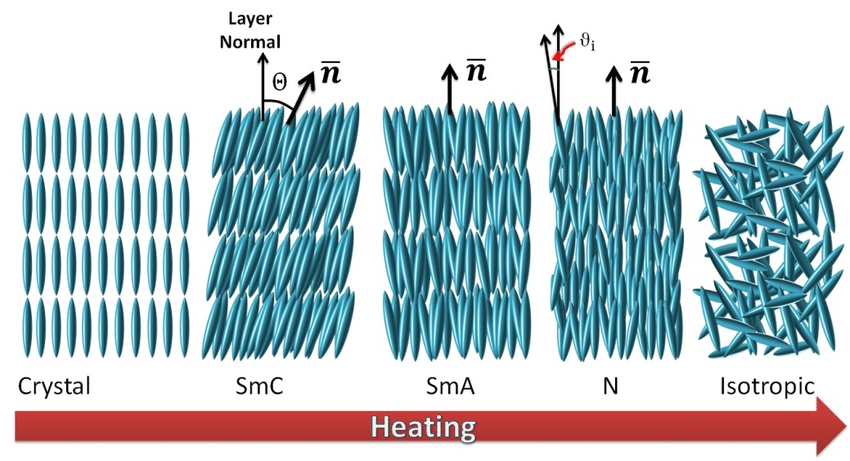
\includegraphics[scale=0.5]{phases.png}
    \caption{\textbf{Multiple mesophases:} \cite{al-zangana_lyotropic_2017} A thermotropic liquid crystal showing two smectic phases (SmC, SmA) and a nematic phase (N) in the transition from crystalline solid to isotropic liquid. Notice the molecular layers present in the smectic phases but not the nematic phase.}
    \label{fig:phases}
\end{figure*}

\begin{figure}
    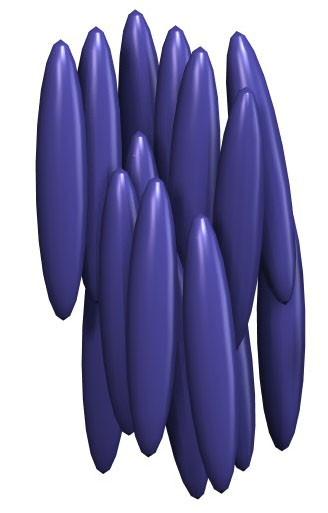
\includegraphics[scale=0.3]{nematic.jpg}
    \caption{\textbf{Uniaxial nematic phase}}
    \label{fig:nematic}
\end{figure}

\begin{figure}
    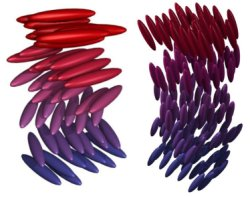
\includegraphics[scale=0.8]{cholesteric.jpg}
    \caption{\textbf{Cholesteric (a.k.a. chiral nematic) phase}}
    \label{fig:cholesteric}
\end{figure}

\begin{figure}
    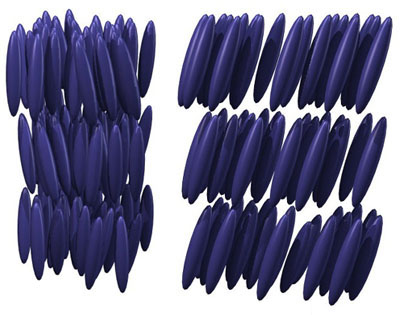
\includegraphics[scale=0.5]{smectic.jpg}
    \caption{\textbf{Smectic A (left) and C (right) phases}}
    \label{fig:smectic}
\end{figure}

\begin{figure}
    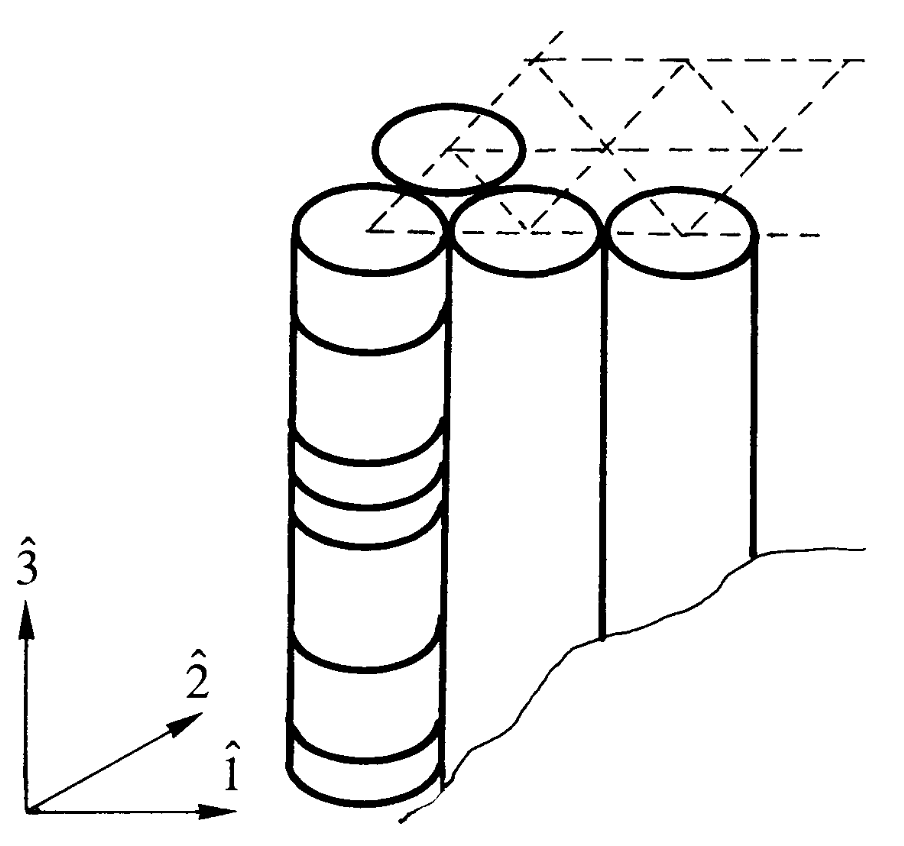
\includegraphics[scale=0.3]{columnar.png}
    \caption{\textbf{Columnar phase:} \cite{gennes_physics_1974} Note the randomness of the intermolecular distance along the columnar axis. }
    \label{fig:columnar}
\end{figure}


\section{Verification of Code}

\subsection{Core Simulation}

I sought to simulate the alignment of liquid crystals to the electric field of a capacitor.  I took a two-pronged approach to this problem: \begin{enumerate}
\item Simulate the electric field of an azimuthally symmetric capacitor using Laplace relaxation
\item Simulate the alignment of liquid crystals to an external electric field using Runge-Kutta methods
\end{enumerate}

\subsubsection{Capacitor Fields via Laplace relaxation}

Gauss's Law in a region with no charge density takes the following form:
$$ \nabla \cdot \mathbf{E} = \frac{\rho}{\varepsilon_0} = 0 $$
\noindent Moreover, since the electric field is the gradient of the electric potential, $\mathbf{E} = \nabla \phi$, we have
$$ \nabla \cdot \nabla \phi = \nabla^2 \phi = 0 $$
\noindent which is Laplace's equation.

We can rewrite the derivatives in $\nabla^2 \phi$ as limits to obtain a finite-difference version of Laplace's equation:
$$ \pdd{\phi}{x} = \lim_{\Delta x \to 0} \frac{\phi(x + \Delta x, y) - \phi(x,y)}{\Delta x} $$
\begin{align*}
	\psdd{\phi}{x}  &=  \lim_{\Delta x \to 0} \frac{\frac{\phi(x + \Delta x, y) - \phi(x,y)}{\Delta x} - \frac{\phi(x, y) - \phi(x - \Delta x,y)}{\Delta x}}{\Delta x} \\ 
	&= \lim_{\Delta x \to 0} \frac{\phi(x + \Delta x, y) + \phi(x - \Delta x, y) - 2\phi(x,y)}{\Delta x^2}
\end{align*}

\noindent and similarly for the $y$-derivatives.  Letting $\Delta x = \Delta y = \Delta$, the Laplace operator in Cartesian coordinates becomes 
\begin{align*}
\nabla^2 \phi ={}& \psdd{\phi}{x} + \psdd{\phi}{y} \\
\begin{split}
    ={}& \lim_{\Delta \to 0} \frac{1}{\Delta^2} \left[\phi(x+\Delta, y) + \phi(x - \Delta, y)\right. \\
         & \left. {} + \phi(x,y+\Delta) + \phi(x,y-\Delta) -4\phi(x,y) \right]
\end{split}
\end{align*}
\noindent Thus, on a grid with finite spacing $\Delta$, Laplace's equation yields
\begin{align*}
\nabla^2 \phi ={}& 0 \\
\begin{split}
   \implies \phi(x,y) ={}& \frac{1}{4} \left[\phi(x+\Delta, y) + \phi(x - \Delta, y)\right. \\
         & \left. {} + \phi(x,y+\Delta) + \phi(x,y-\Delta) \right]
\end{split}
\end{align*}
\noindent that is, the potential at each grid point is the average of the potentials at its four nearest neighbors.

This relation can be used to iteratively solve Laplace's equation in free space: specifically, we update the value of $\phi(x,y)$ using its neighbors' values from the previous iteration.  Let $\phi_n$ denote the value of $\phi$ at the $n$'th iteration.  The update rule is then
\begin{align*}
\begin{split}
   \phi_{n+1}(x,y) ={}& \frac{1}{4} \left[\phi_n(x+\Delta,y) + \phi_n(x-\Delta,y)\right. \\
         & \left. {} + \phi_n(x,y+\Delta) + \phi_n(x,y-\Delta) \right]
\end{split}
\end{align*}

\begin{figure}
    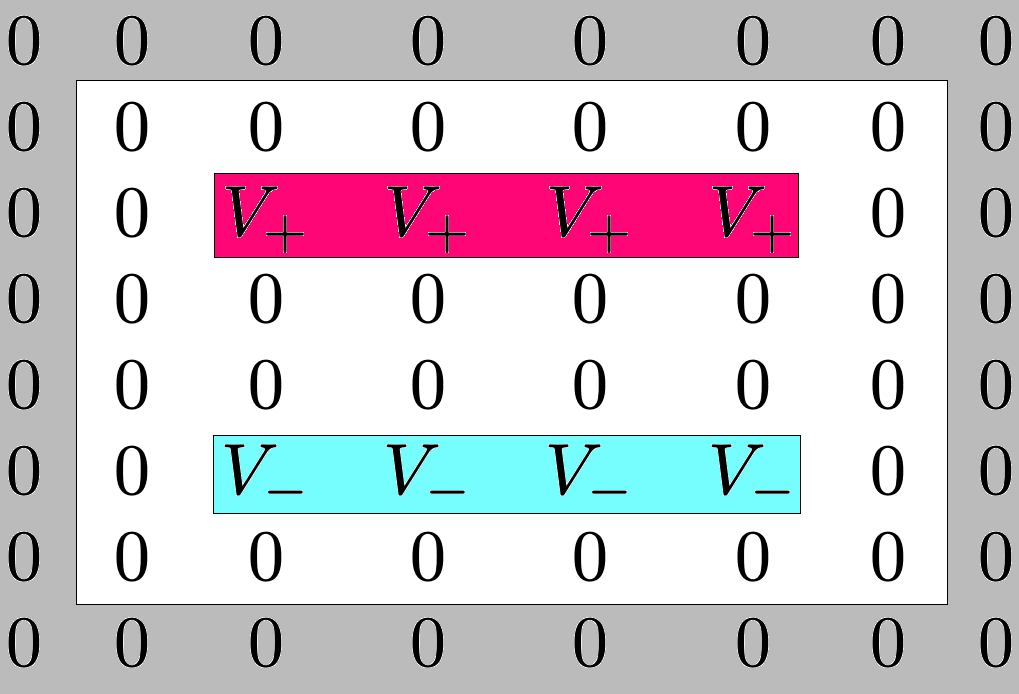
\includegraphics[width=\columnwidth]{cap4.png}
    \caption{\textbf{Finite-element capacitor:} After each iteration of Laplace relaxaton, the potential is set to $V_+$ and $V_-$ on the upper and lower plates (red and blue) and to 0 on the bounding box (grey).  The values in the white background change with each iteration.}
    \label{fig:cap}
\end{figure}

Now we consider boundary conditions that enable us to solve the equation in closed form.  We want to find the electric field of a capacitor with plates at constant potential $V_+$ and $V_-$.  Following the convention that the potential is zero at infinite distance from the capacitor, we place the capacitor in a grounded (i.e., $\phi=0$) bounding box far enough away that it does not affect the $\mathbf{E}$ field inside the capacitor.  We impose these conditions by resetting the grid points representing the capacitor plates and bounding box after each iteration (Fig. \ref{fig:cap}).

Finally, we need to adapt the method to handle azimuthally symmetric 3D capacitors.  ``Azimuthal symmetry'' just means that the potential is independent of $\theta$ when expressed in cylindrical coordinates: $\phi(r,\theta,z) = \phi(r,z)$.  In other words, the system is invariant under rotations around the $z$-axis.  This means we can continue to use the 2D Laplace relaxation method without having to add a third variable.

In cylindrical coordinates, the Laplacian is \cite{arfken_mathematical_2013}
\begin{align*}
	\nabla^2 \phi(r,z) &= \frac{1}{r} \pd{r} \left(r \pdd{\phi}{r}\right) + \frac{1}{r^2} \psdd{\phi}{\theta} + \psdd{\phi}{z} \\
	&=  \frac{1}{r} \pd{r} \left( r \pdd{\phi}{r}\right) +  \psdd{\phi}{z} 
\end{align*}
Expanding the $r$-derivative into limits gives
\begin{align*}
\frac{1}{r} \pd{r} \left( r \pdd{\phi}{r}\right) &={} \frac{1}{r} \left( \pdd{\phi}{r} +r \psdd{\phi}{r} \right) \\
&={} \frac{1}{r} \pdd{\phi}{r} + \psdd{\phi}{r} \\	
\begin{split}
&={} \lim_{\Delta r \to 0} \left(  \frac{\phi(r + \Delta r, z) - \phi(r,z)}{r \Delta r} \right. \\
         &{} \left. {}+ \frac{\phi(r + \Delta r, z) + \phi(r-\Delta r, y) - 2\phi(r,z)}{\Delta r^2} \right)
\end{split}
\end{align*}
or, using the symmetric difference $$\frac{\phi(r+\Delta r, z) - \phi(r - \Delta r, z)}{2 \Delta r}$$ for $\partial \phi / \partial r$,
\begin{align*}
\begin{split}
    \frac{1}{r} \pd{r} \left( r \pdd{\phi}{r}\right) ={}& \lim_{\Delta r \to 0} \left(  \frac{\phi(r + \Delta r, z) - \phi(r - \Delta r,z)}{2 r \Delta r} \right. \\
         &\left. {}+ \frac{\phi(r + \Delta r, z) + \phi(r-\Delta r, z) - 2\phi(r,z)}{\Delta r^2} \right) \\
\end{split}
\end{align*}

Combining this with the finite-difference $z$-derivative and letting $\Delta r = \Delta z = \Delta$, we get

\begin{align*}
\nabla^2 \phi(r,z) &={} \frac{1}{r} \pd{r} \left(r \pdd{\phi}{r}\right) + \psdd{\phi}{z} \\
\begin{split}
&={} \lim_{\Delta \to 0} \bigg(  \frac{\phi(r + \Delta, z) - \phi(r - \Delta,z)}{2 r \Delta} \\
&+\frac{1}{\Delta^2}\big[\phi(r + \Delta, z) + \phi(r-\Delta, z) \\
&+ \phi(r, z + \Delta) + \phi(r, z - \Delta) - 4\phi(r,z)\big] \bigg) \\
\end{split}\\
\end{align*}

This gives the update rule

\begin{align*}
\begin{split}
   \phi_{n+1}(r,z) ={}& \frac{1}{4} \bigg[ \left(1 + \frac{\Delta}{2r}\right)\phi_n(r+\Delta,z) \\
   &{} + \left( 1 - \frac{\Delta}{2r}\right)\phi_n(r-\Delta,z) \\
         &  {} + \phi_n(r,z+\Delta) + \phi_n(r,z-\Delta) \bigg]
\end{split}
\end{align*}

One last subtlety in the azimuthal case is that $r$ cannot be allowed to be 0 since the $\Delta / 2r$ term in the update will diverge.  To solve this, we discretize $r$ as $$r \in \left\{\frac{\Delta}{2}, \frac{\Delta}{2} + \Delta, \frac{\Delta}{2} + 2 \Delta, \dots \right\}$$

\subsubsection{LC Alignment via Runge-Kutta}

I modeled the LC molecule as a dipole consisting of two masses with opposite charges connected by a rigid, massless rod.  The total force on each of the two charges is made up of the electric force due to the field, the restoring force due to the tension in the rod, and the drag from the viscosity of the solution.  Thus, we can write the force on the two charges $\oplus$ and $\ominus$ as
$$ \mathbf{F}_\oplus = m\ddot{\mathbf{x}}_\oplus = q_\oplus\mathbf{E}(\mathbf{x}_\oplus) - k(r-r_0)^2\hat{\mathbf{r}} - \beta \dot{\mathbf{x}}_\oplus $$
$$ \mathbf{F}_\ominus = m\ddot{\mathbf{x}}_\ominus = q_\ominus\mathbf{E}(\mathbf{x}_\ominus) + k(r-r_0)^2\hat{\mathbf{r}} - \beta \dot{\mathbf{x}}_\ominus $$
\noindent where: 
\begin{list}{}{}
\item $\mathbf{x}$, $\dot{\mathbf{x}}$, and $\ddot{\mathbf{x}}$ are respectively the position, velocity, and acceleration of the charge;
\item $m$ is its mass;
\item $q$ is its charge;
\item $\mathbf{E}(\mathbf{x})$ is the electric field at position $\mathbf{x}$;
\item $k$ is a spring constant;
\item $\mathbf{r} = \mathbf{x}_\oplus - \mathbf{x}_\ominus$, $r = |\mathbf{r}|$, and $\hat{\mathbf{r}} = \mathbf{r}/r$; 
\item $r_0$ is the equilibrium separation between the two charges; and
\item $\beta$ is a damping constant representing the viscosity of the solution.
\end{list}
Defining $\mathbf{v} = \dot{\mathbf{x}}$, we can de-couple the two second-order equations into four first-order equations:
\begin{align*}
	\dot{\mathbf{x}}_\oplus &= \mathbf{v}_\oplus \\
	\dot{\mathbf{v}}_\oplus &= \frac{1}{m_\oplus}\left[q_\oplus\mathbf{E}(\mathbf{x}_\oplus) - k(r-r_0)^2\hat{\mathbf{r}} - \beta \mathbf{v}_\oplus\right] \\
	\dot{\mathbf{x}}_\ominus &= \mathbf{v}_\ominus \\
	\dot{\mathbf{v}}_\ominus &= \frac{1}{m_\ominus}\left[q_\ominus\mathbf{E}(\mathbf{x}_\ominus) + k(r-r_0)^2\hat{\mathbf{r}} - \beta \mathbf{v}_\ominus\right]
\end{align*}
These equations are nonlinear whenever $r_0 \neq 0$ or $\mathbf{E}(\mathbf{x})$ is nonlinear, so they are best solved numerically.  I solved them using the 4th-order Runge-Kutta method, which I will not explain here.

\subsection{Verification}

\subsubsection{Capacitor Fields}
To verify the code for the capacitor field calculation, I set up two constant-potential plates with opposite charges and calculated the potential in the region surrounding them.  Then I took slices at constant z-values and graphed the resulting two dimensional potential $\phi(r)=\phi(x,y)$ in the $x$- and $y$-axes using a heatmap.  For comparison, I also made a simple $r$-vs.-$\phi(r)$ graph for each slice.

Between the two plates, we expect the potential to decrease linearly from $V_{+}$ to $V_{-}$ as we move from the negative to the positive plate.  Additionally, if we start in between the plates and increase $r$ until we move outside of the ``dielectric'', we expect to see the potential drop to 0 in approximately as $1/r^2$.  Moreover, if we start between the plates and change $z$ until we leave the space between the plates, we should see the potential fall to 0 even more quickly than $1/r^2$ due to shielding effects.

In the verification simulation, capacitor plates are placed $z=200$ and $z=300$ and slices are taken at $z=200$, $z=250$, and $z=300$.  Figures \ref{top_plate}, \ref{fig:between_plates}, and \ref{fig:bottom_plate} show the expected behavior described above.  In addition, adjusting the $z$ range such that slices are calculated for $z<200$ and $z>300$ shows the potential quickly returning to zero as expected (see iPython notebook).

\begin{figure*}
	\centering    
    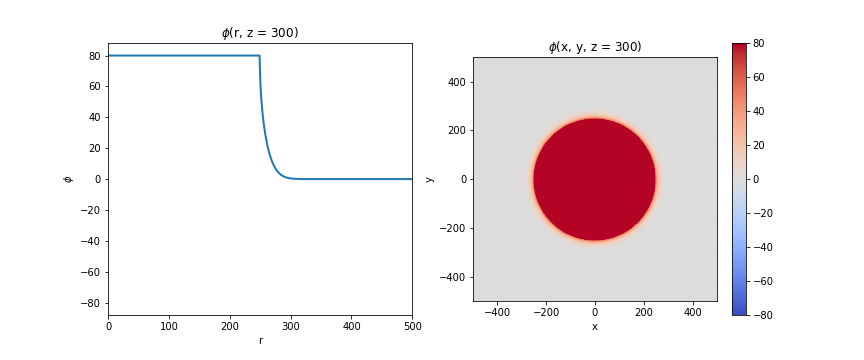
\includegraphics[scale=0.52]{top_plate.png}
    \caption{\textbf{Top plate:} The top plate located at $z=300$ has constant potential $V_+ = +80$. }
    \label{fig:top_plate}
\end{figure*}

\begin{figure*}
	\centering    
    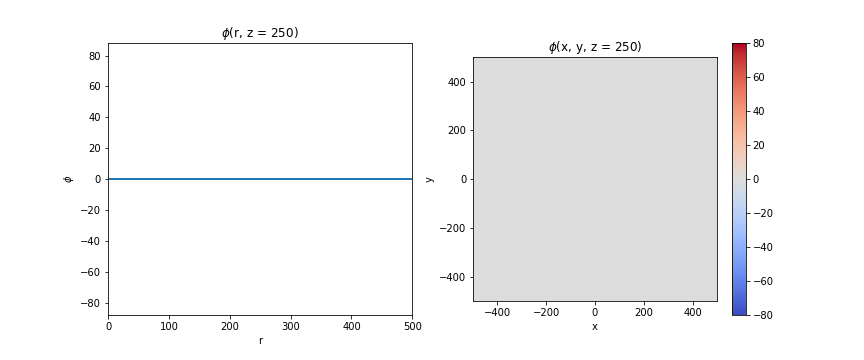
\includegraphics[scale=0.52]{between_plates.png}
    \caption{\textbf{Between plates:} At $z=250$, the $\textbf{E}$ fields of the top and bottom plate cancel and $\phi(r) = 0$ everywhere. }
    \label{fig:between_plates}
\end{figure*}

\begin{figure*}
	\centering    
    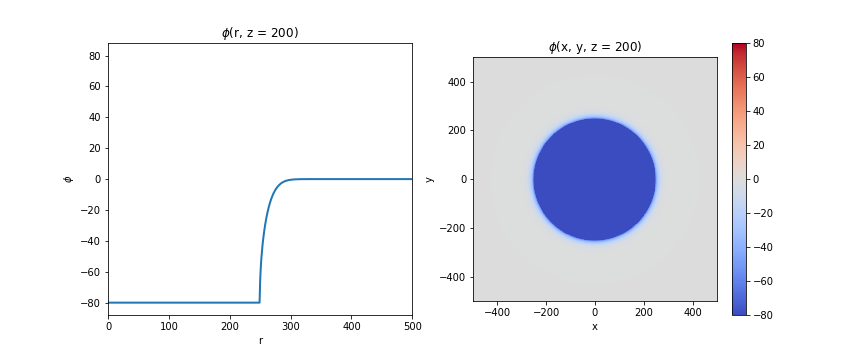
\includegraphics[scale=0.52]{bottom_plate.png}
    \caption{\textbf{Bottom plate:} The bottom plate located at $z=200$ has constant potential $V_- = -80$. }
    \label{fig:bottom_plate}
\end{figure*}

\subsubsection{LC Alignment}
To verify the code for the dipole alignment calculation, I set up a single dipole angled at $45^{\circ}$ relative to a constant electric field in the $+z$ direction.  In the absence of viscosity (i.e., $\beta = 0$), the dipole should oscillate about the equillibrium position indefinitely like a frictionless pendulum.  With nonzero $\beta$, the amplitude of oscillations should decrease until the dipole is at rest and aligned with the field, similar to a damped pendulum.  

Figure \ref{fig:dipole} shows the behavior described above.

\begin{figure}
	\centering    
    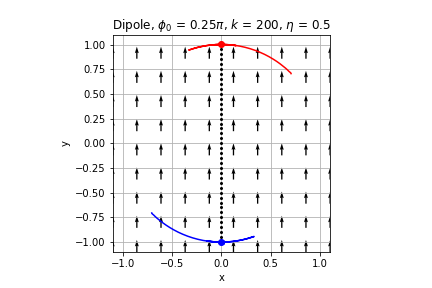
\includegraphics[width=\columnwidth]{dipole_rest.png}
    \caption{\textbf{Dipole at rest:} The red and blue curves track the motion of the charges from $45^{\circ}$ offset relative to the field at $t=0$ to aligned with the field at rest for $t\to \infty$. }
    \label{fig:dipole}
\end{figure}

\section{Discussion and Future Work}

Although I have only presented the verification of code with simple cases, the functions in the associated iPython notebook are more flexible.  In the notebook I submitted with this report, I have configured the capacitor calculations with radially varying charges on the electrodes.  Also, the dipole simulation can take an arbitrary user-defined 2D electric field instead of the constant field I used for demonstration.

I plan to work more on this project this summer.  Specifically, I plan to more accurately simulate an ensemble of liquid crystals in the electric field of a general 3D potential $\phi(r,\theta,z)$.  I emphasize cylindrical configurations because they apply most readily to simulating liquid crystal lenses, which I want to do because of my interest in adaptive optics.

\section{Acknowledgements}
I would like to thank Prof. Blas Cabrera and all of the teaching staff for teaching PHYSICS 113 this quarter in spite of the unprecedented circumstances.  I especially thank Stan Fort and Emily Been for answering my questions related to class material and this project.  I learned this quarter that you don't need a laboratory to do physics experiments, you just need a little bit of Python and a lot of patience!

%\vspace{5mm}
%The code related to this project can be found at \url{https://github.com/murphyjm/phys108}.

\bibliography{biblio}


\end{document}

%sagemathcloud={"latex_command":"latexmk -pdf -f -g -bibtex -synctex=1 -interaction=nonstopmode '2017-01-27-111544.tex'"}